\chapter{Techniques}
\label{Chapter4}
\lhead{Chapter 4. \emph{Codes}}

Throughout this thesis, my goals were to identify SLSNe in a number of surveys. I have approached this problem using a number of tools and techniques, each playing an important role in achieving this goal. The aim of this chapter is to provide an overview of the methods used in this work. I begin by discussing my approach to the modelling of SLSNe using the popular spin-down of a magnetar model \sref{sec:SLAP}. I describe the model and the improvements I have introduces in order to better model the UV region of the SLSN SED. I also describe the fitting routines used in the modelling of SLSNe (and other projects as part of this thesis). While this technique was successful in reproducing the light curves of SLSNe as well as identifying a new SLSN in the SNLS, it was not robust enough to fully capture the diversity of the SLSN sample and was not sufficient to classify SLSNe by itself. To solve this problem, I followed an increasingly popular approach of applying the state-of-the-art Machine Learning (ML) techniques to automate the classification process. The later parts of this chapter focus on the techniques and software developed in order to build the training sample of SNe and other transients required for this study, described in \cref{Chapter5}.

The use of ML moves the focus of this work away from understanding the parameter spaces of the SLSN models, or the choice of cuts needed to define them. Instead, I focus on simulating transients and their detectability in DES. This includes SNIa, hydrogen-poor (SNIb/c) and rich CCSNe (SNII), SLSNe, AGNs as well as random noise spikes which are the main source of contamination in the data. The models of SN\,Ia are mature and ready to be deployed in this work \citep{Kessler2009,Kessler2015} thanks to being used as cosmological probes for over two decades \citep{Riess1998,Perlmutter1999}. Simulations of CCSNe, however, not driven by similar motivations as SNIa, have not been developed equally extensively, becoming one of the key subjects of this thesis. CCSNe are usually more rapidly evolving and fainter than SNIa, resulting in a significantly smaller sample of well-observed objects. The number of objects with a high-quality spectroscopic follow-up is also much lower in comparison. In recent years, the interest in modelling these objects has increased dramatically with large surveys, such as LSST, requiring samples of fake transients in order to inform the design of their observing strategies. In this chapter, I describe our approach to creating a new set of spectroscopic templates for  CCSN as well as simulating them in a number of surveys. This project was build to provide a sample of stripped-envelope CCSNe as part of the LSST photometric lightcurves classification challenge. However, later I have extended its use to DES in order to create samples of both hydrogen-rich and poor CCSNe.

The last, but perhaps the most important, technique described in this chapter is Gaussian Process Regression (GPR). DES, like to other transient surveys, does not support a stable and uniform cadence of observed making the data incompatible with the majority of ML techniques that require evenly samples data. I used GPR as a method for interpolating the light curves using a non-parametric approach which does not introduce any physically motivated biases in the fitting process. This is key to solving the overfitting problem, often encountered when working with relatively small training sample within ML framework.

This chapter is divided in the following way: I begin by describing the methods behind the modelling of SLSNe using the magnetar model as well the extensions I have introduced alongside the SED corrections in the UV. Next, I discuss the packages and techniques developed in order to model SN\,Ib/c as well as SNII. Finally, I describe GPR as a non-parametric approach to interpolating light curves.

\section{Modeling SLSN Light Curves} \label{sec:SLAP}
Throughout this thesis, the modelling of SLSNe light curves plays a pivotal role. The measurement of the rate of SLSNe presented in \cref{Chapter3}, as well as the search for SLSNe in DES, described in \cref{Chapter5,Chapter6} uses a definition of SLSNe based on the spin-down of the magnetar model. This choice comes after a simpler model, describing SLSNe using a linearly expanding and cooling photosphere, was tested but eventually rejected in favour of the magnetar model. I introduce this basic model, including its drawbacks, before I describe the magnetar model. I also outline the improvements introduced to the modelling of the SED of SLSNe.

When modelling light curves of SLSNe there are two independent, but equally important, areas that contribute to the accuracy of the model: the SED of the SN, and its evolution with time. The need to model the SED of a SN could be avoided if we used an approach which purely relied on the bolometric lightcurves as opposed to multi-band observations. From the implementation point-of-view, these models are easier to use and are common in the literature \citep{Inserra2013,Papadopuplus2014,Nicholl2014}. However, they do not consider the colour, along with its evolution, of a SN which provides a very powerful tool for further constraints on the properties of the SNe. It has been previously shown \citep{Chomniuk2011,Howell2013,Papadopuplus2014,Vreeswijk2014} that the SLSN SED can be accurately approximated, in the visible spectrum, by a slowly evolving blackbody with an addition of their characteristic broad absorption lines of O\,II. However, this approximation breaks down in the near UV due to the prominent broad absorption features which can be attributed to Mg\,II, Fe\,III, C\,II, Co\,III, Si\,III and Ti\,III \citep[see][for line identifications]{Mazalli2016}.

\subsection{Improving the blackbody approximation} \label{sec:KCorrection}
In order to improve the modelling of the SLSN SED, I propose a method of improving the blackbody approximation by superimposing absorption template onto the simple blackbody SED. In order to derive these template, I use a method similar to that of  \citet{Vreeswijk2014} where I fit the Planck function to several featureless, 50$\AA$ wide regions of the spectrum in order to measure the underlined blackbody continuum in the SED, as shown in figure \ref{fig:specTemplate}. The resulting fits show that the absorption relative to the blackbody is low in the regions of $\lambda>3000\AA$, and increases drastically in the bluer regions of the spectrum.

The time evolution of the spectra appears to be weak in comparison to other SNe, making it possible to approximate the SED at any epoch using the Planck function, where the temperature evolves with time, and a single absorption template is used. The absorption is calculated as a ratio of the observed flux to the continuum blackbody fit. The number of SLSNe with good UV coverage remains small, with only the spectra of iPTF13ajg \citep{Vreeswijk2014}, SCP06F6 \citep{Barbary2009} and SNLS-06D4eu \citep{Howell2013}. Do due to the observer-frame coverage of their respective spectra, our spectral templates cover a rest-frame wavelength range of 1620--3320\,\AA\ (SNLS-06D4eu), 1800--3800\,\AA\ (SCP06F6) and 1800--5250\,\AA\ (iPTF13ajg).

\begin{figure}
\centering
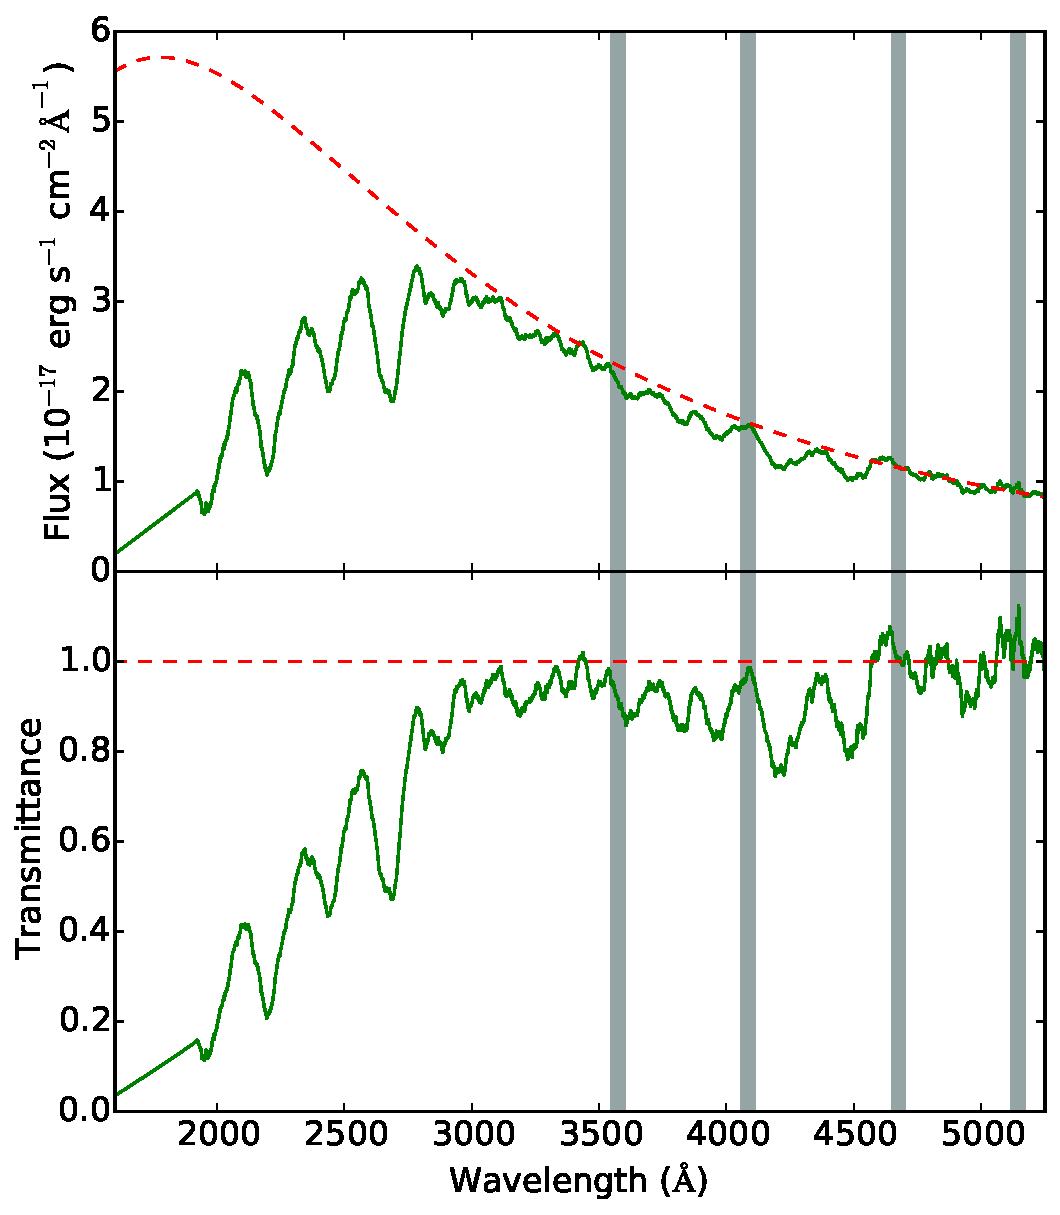
\includegraphics[width=\textwidth]{Figures/Chapter4/specTemplate}
\caption{iPTF13ajg is fitted with the Planck function. The spectrum of iPTF13ajg (green) can shows a good agreement with the blackbody (red) at $\lambda>3000\AA$. At lower wavelengths a strong deviation from the model is observed, highlighting the need for a correction to the model. The ratio between the observed spectrum and the continuum give a measure of the absorption strength as a function of wavelength and can be used in modelling the SLSN SED.}
\label{fig:specTemplate}
\end{figure}

\subsection{Modelling the SED evolution}
The ability to describe the SEDs of SLSNe as blackbodies greatly simplify the
modelling of its evolution. A model is only required to provide the thermal and radial evolution of the photosphere, therefore removing the need for complex modelling such as radiative transfer or hydrodynamic simulations.

\subsubsection{Fireball model}
Perhaps the simplest approach to modelling the SED evolution is to assume that the SN, with an initial radius R$_{0}$ and initial temperature T$_{0}$ expands at a constant rate while cooling down also at a current rate as seen in \eref{eq:Howell}
\begin{align}
\label{eq:Howell}
R(t) &= R_0 + \dot{R}t &&\\
T(t) &= T_0 - \dot{T}t &&
\end{align}
\noindent While this model is not physical motivated, \citet{Howell2013} showed that it provides a good, first-order approximation to the light-curves of SLSNe. Due to its simplicity, the model appeared as an attractive prospect for the modelling of SLSN SEDs. However, our testing showed that while it produces a good fit to a SLSN around the maximum light (<+30days) it is not able to capture the slow evolution in the tale of the light curve as seen in \fref{fig:BB_Mag} making in unfavourable in comparison with the more complex magnetar model.

\begin{figure}
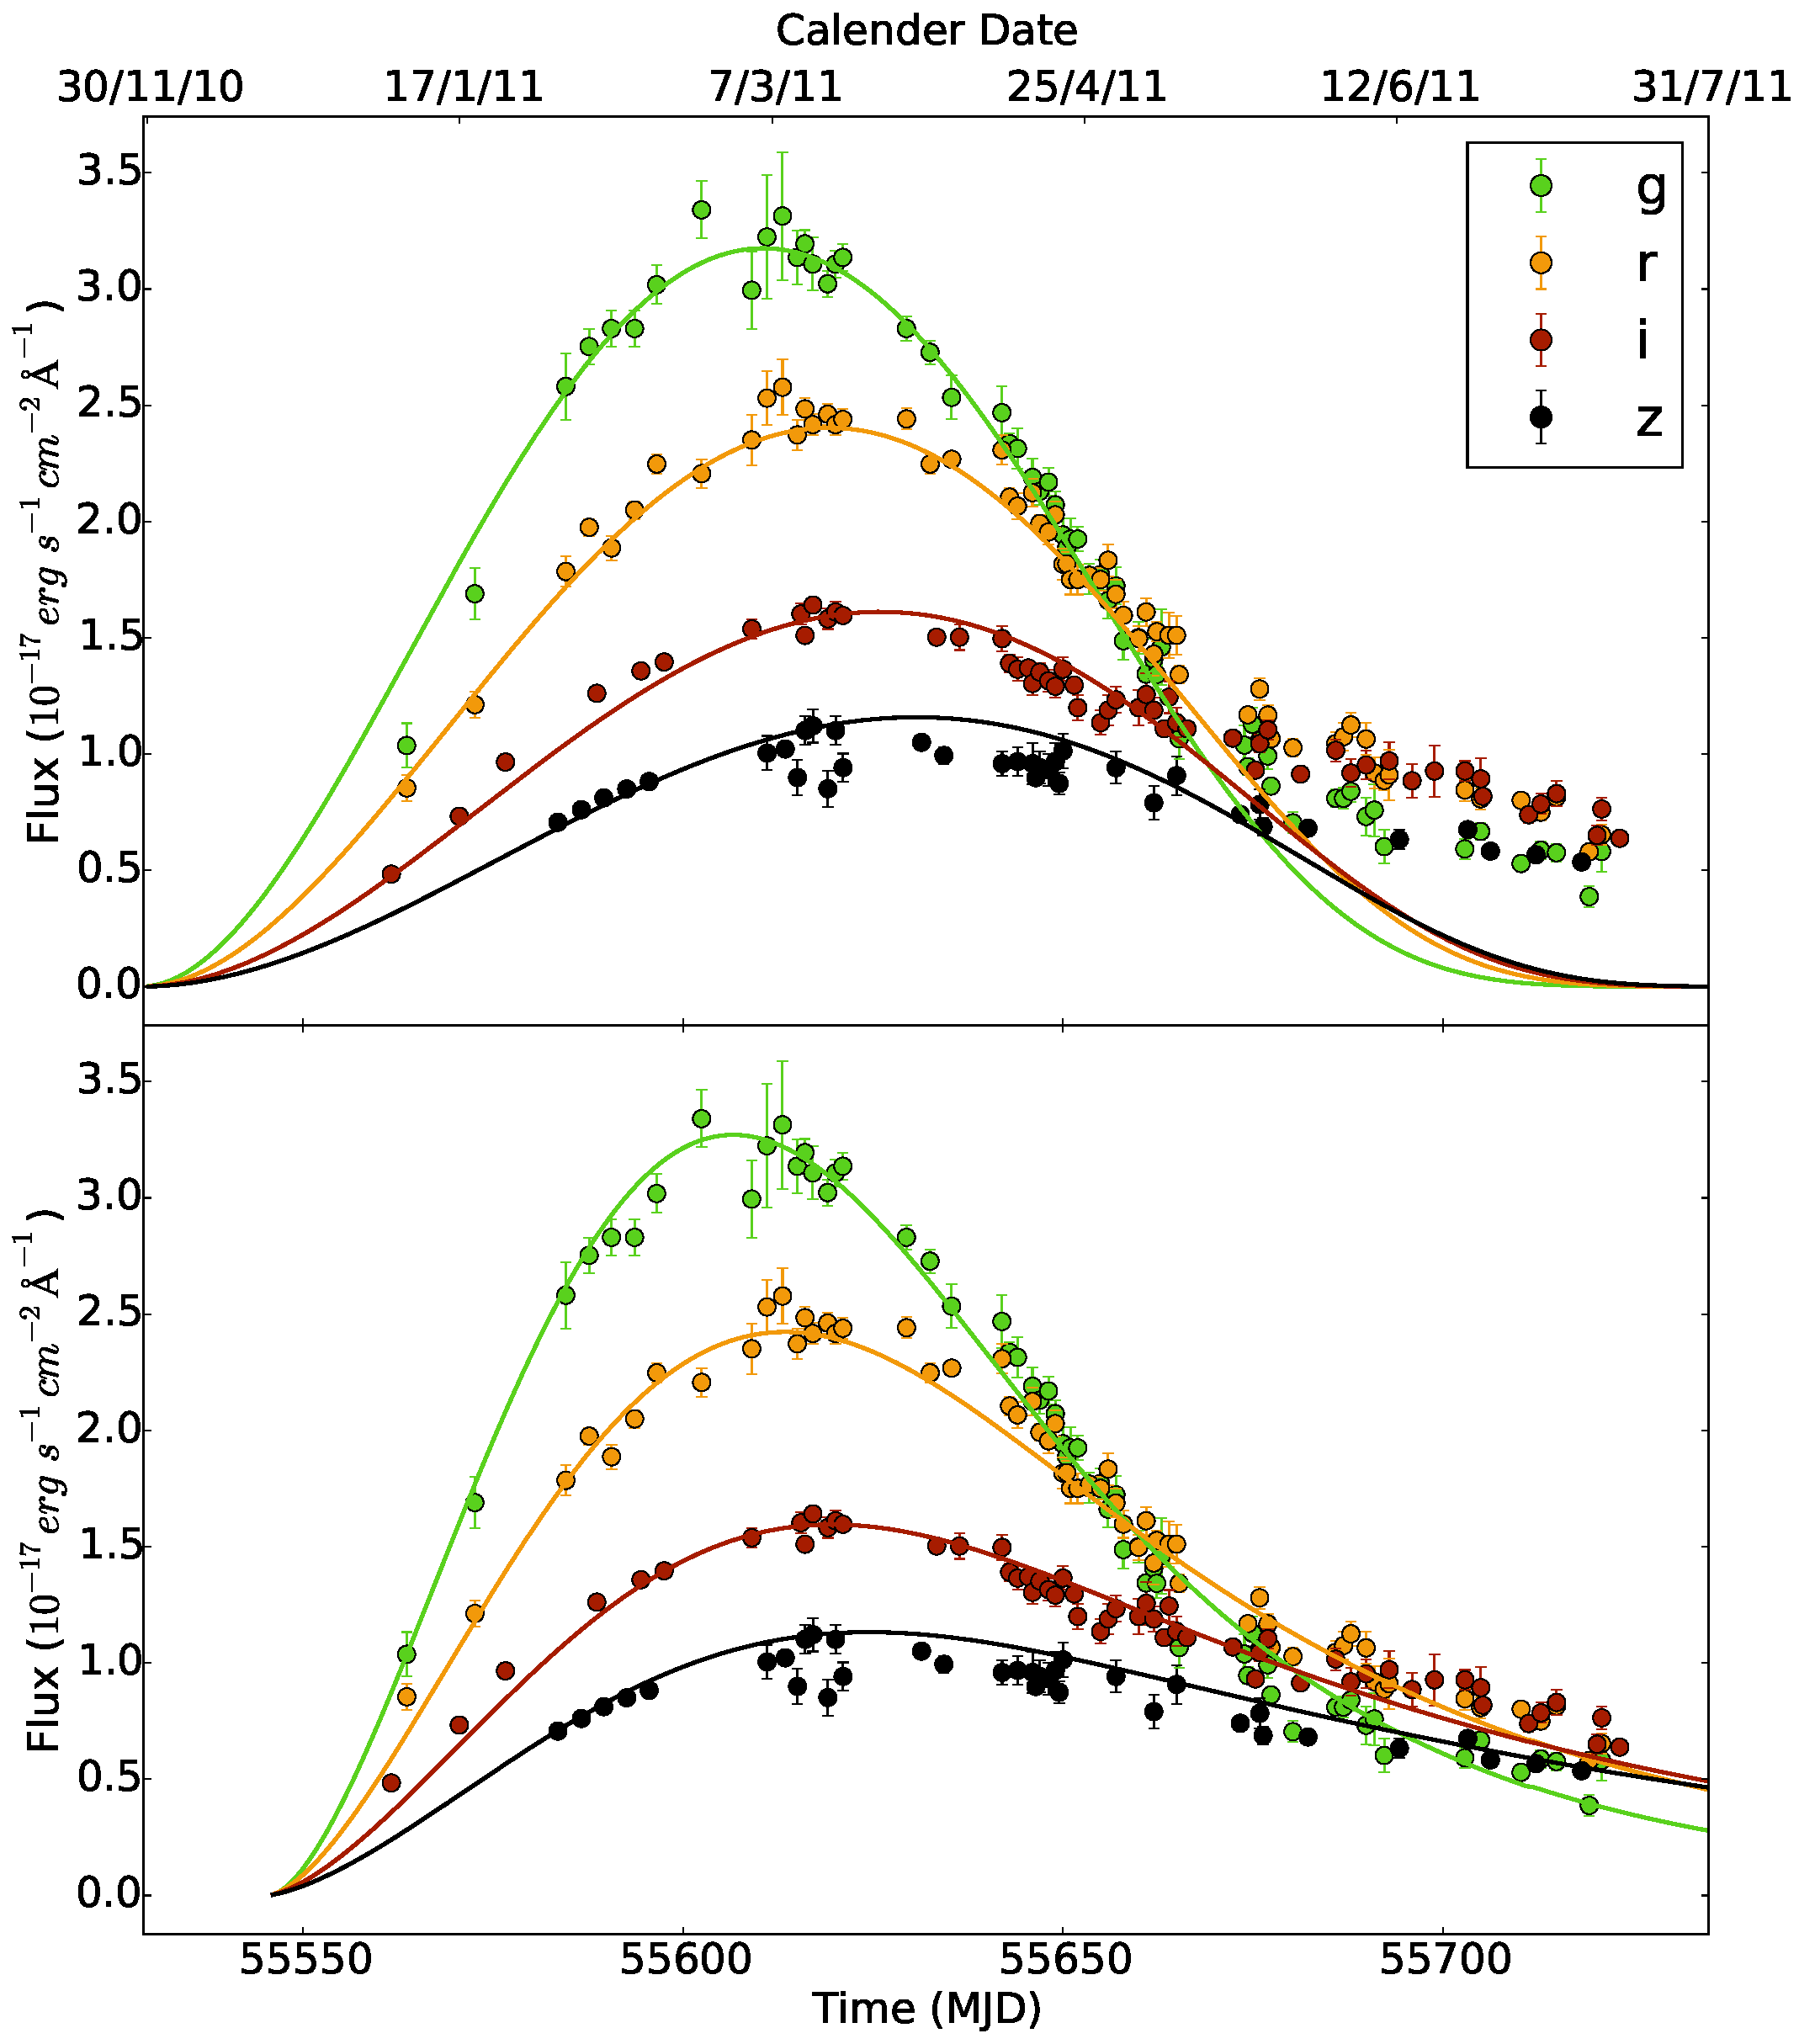
\includegraphics[width=\textwidth]{Figures/Chapter4/BB_Mag_comp}
\caption{The SLSN PS1-11ap $griz$ light curve \citep{McCrum2014} compared to two models describing its photometric evolution. In the upper panel, the model is a simple expanding and cooling blackbody fitted to data around maximum light only, and in the lower panel, the model is our `absorbed' magnetar model fitted to the entire light curve. In the case of the magnetar model, the spectrum of SNLS-06D4eu \citep{Howell2013} has been used as an absorption template in the modelling of the SED \sref[see]{sec:KCorrection}). Note that while both models can produce reasonable fits around the peak of the light cuve, the black body model is not able to reproduce the characteristic late-time behaviour of SLSNe. Light curve phases are measured with respect to peak brightness in the rest-frame \textit{u}-band as predicted by our magnetar model fit.}
\label{fig:BB_Mag}
\end{figure}

\subsubsection{Magnetar model}
\label{sec:Magnetar}
To fully capture the evolution of the SED with time we must employ a model for an engine that provides the late time energy deposition needed to explain the photospheric velocity and temperature observed in SLSNe. While still a matter of active debate in the literature, in recent years the birth and spin-down of a magnetar model have appeared as the strongest candidate to explain these extremely luminous events \citep{Inserra2013,Nicholl2013}. In this model, SLSNe begin as CCSNe with a magnetar, a rapidly rotating, highly magnetised neutron star, born at its core. As the magnetar spins down due to the interactions with its environment, it dissipates its energy in the form of high energy radiation that is then captured by the expanding ejecta and thermalised to produce the observed blackbody SED \citep{Kasen2009,Woosley2010,Inserra2013}.

I follow the method from \citet{Inserra2013}, based on the Arnett law for the energy diffusion through SN ejecta \citep{Arnett1982}, and the energy radiated by the central engine from \citet{Bildsten2013,Wosley2012}. In order to model the bolometric luminosity, $L$, of a SLSN as a function of time, $t$, we use equation \ref{Eq:MagnetarLum}:
\begin{equation}
L(t) = 4.9\times 10^{46}\,e^{ -(t / \tau_\mathrm{m})^2 }\delta(t) \int_{0}^{t} \frac{2t'}{\tau_\mathrm{m}^2}\,e^{(t'/\tau_\mathrm{m})^2}\,\frac{B_{14}^{2}\,P_{\mathrm{ms}}^{-4}}{\left(1+t'/\tau_\mathrm{p}\right)^2} dt',
\label{Eq:MagnetarLum}
\end{equation}
\begin{equation}
\label{Eq:SDPeriod}
\tau_{p} = 4.7B_{14}^{-2}P_{ms}^{2}days
\end{equation}
\noindent where $\tau_\mathrm{m}$ is the diffusion timescale, $B_{14}$ is the neutron star magnetic field in units of $10^{14}$\,G, $P_{\mathrm{ms}}$ is the magnetar spin period in ms, $\delta(t)$ is the deposition function or trapping coefficient, and $\tau_\mathrm{p}$ is the magnetar spin-down timescale, is defined in \eref{Eq:SDPeriod}, inferred from $B_{14}$ and $P_{\mathrm{ms}}$.

Physically $\tau_M$ is proportional to the ejecta mass($M_{ej}$) which is sometimes chosen as the fit parameter instead. The two parameters can be interconvert using equation \ref{Eq:Mej}, where $E$ is the explosion energy and $\kappa$ the opacity of ejecta.
\begin{equation}
\label{Eq:Mej}
M_{ej} = (\frac{\tau_{M}}{10days})^{4/3}(\frac{\kappa}{0.1cm^2g^{-1}})^{-2/3}(\frac{E_k}{10^{51}erg})^{1/3}M_{\odot}
\end{equation}
\noindent It has been shown \citep{Inserra2013,Inserra2014,Nicoll2015,Papadopuplus2014} that the opacity and the explosion energy parameters have only a weak affect the quality of fitting and have therefore been fixed as $\kappa = 0.1cm^2g^{-1}$ and $E = 10^{51}$erg respectively.

The velocity of the ejecta, $v_{core}$ are assumed to be constant and value can be found using the inferred mass of the ejecta, $M_{ej}$ and its kinetic energy, $E_{mag}$ (\eref{Eq:vcore}), which in turn depends on the explosion energy and the energy released by the spin down of the magnetar, shown in \eref{Eq:Emag}:
\begin{align}
\label{Eq:Emag}
E_{mag} = 4.9\times10^{46} B^2 P^{-4} \tau_{P}  \text{ erg} \\
E_k = 10^{51} + 0.5 \times E_{mag} \text{ erg}\\
\label{Eq:vcore}
v_{core} =  \sqrt{\frac{10 E_{k}}{3 M_{ej}}} \text{ cm s}^{-1}
\end{align}

\paragraph{Trapping coofficient}
The trapping coefficient, $\delta(t)$, is defined as the fraction of the high-energy radiation produced by the central engine that gets trapped, and subsequently reproduced as visible light, by the ejecta. It is often assumed in the literature that the trapping coofficient is time-independent and close to unity, implying the full trapping of radiated by the supernova ejecta \citep{Inserra2013,Papadopuplus2014,Nicoll2015}. In this work I use a correction introduced by \cite{Wang2015} with a time-dependent trapping coefficient:
\begin{equation}
\delta(t) = 1 - \exp\left({-\frac{9\kappa \mathrm{M}_{\mathrm{ej}}^{2}}{40\pi  E_k} t^{-2}} \right),
\label{Eq:Wang}
\end{equation}
\noindent where $\mathrm{M}_{\mathrm{ej}}$ is the ejecta mass, $E_k$ is the explosion energy, and $\kappa$ is the opacity. $\mathrm{M}_{\mathrm{ej}}$ is proportional to $\tau_\mathrm{m}$, $E_k$ and $\kappa$ \citep{Inserra2013}. We again fix the explosion energy to be $E_k = 10^{51}$\,erg and the opacity as $\kappa = 0.1$\,cm$^2$g$^{-1}$.

Using this time-dependent trapping coefficient improves the late-time fit to the light curve. For a typical SLSN we calculate $\delta \simeq 1$ up to 75 days post-explosion. However, as the ejecta opacity to high energy photons decreases with time we find $\delta \simeq 0.8$ at 150 days post-explosion, emphasising the importance of this correction in the late time light curves.

\paragraph{Deriving Radius and Temperature}
In its simplest form, the magnetar model only predicts the total radiated energy of the SN and does not make any predictions about the SED of the object. It is therefore most commonly used with bolometric light curves, synthesised from the photometry. \citet{Inserra2013}, however, shows that it is possible to predict the photospheric radius of a SN based on this model deriving the following equations:
\begin{equation}
\label{Eq:R19}
R(t) = r_{core}(t) \left(\frac{\alpha - 1}{\tau_{core}(t)}\right)^\frac{1}{1 - \alpha}
\end{equation}
\noindent while the radius of the photosphere exceeds that of the core ejecta, and;
\ref{Eq:R20}.
\begin{equation}
\label{Eq:R20}
R(t) = r_{core}(t) - \frac{1 - \frac{\tau_{core}(t)}{\alpha - 1}}{\kappa \rho_{core}(t)}
\end{equation}
\noindent when the photosphere recedes into the core. $r_{core}(t)$, $\rho_{core}(t)=$ and $\tau_{core}(t)$ are defined as follows:
\begin{align}
r_{core}(t) = v_{core}  t \\
\rho_{core}(t)= \frac{3 M_{ej}}{4  \pi  r_{core}^3(t)}\\
\tau_{core}(t) = \kappa  \rho_{core}(t) v_{core} t
\end{align}

Combining this with the total luminosity and assuming that the object radiates as a uniform, spherical blackbody gives us the photospheric temperature. This can be injected into the Planck law to give an approximation for the SED of a SLSN. This method allows for the magnetar model to be fitted directly to the multi-band photometry without the need to produce the pseudo-bolometric light curves. We combine this with the absorption templates to produce a model of the SLSN spectral evolution as a function of time.

\subsection{SLAP}
Upon establishing an approach for modelling SLSNe it was important to encapsulate it in a software package capable of performing under a number of situations. In this thesis, the magnetar model was used in fitting the light curves of both confirmed SLSNe as well as a variety of transients, the majority of which were not SLSNe and could not be well described using this model. We have also used it to simulate SLSN in SNLS as well as produce an artificial training sample for their search in DES.

The code had to satisfy the following requirements:
\begin{itemize}
  \item Fit the magnetar model to all literature SLSNe and estimate their parameters.
  \item Perform a successful fit to any light curve and return an output, regardless of whether it is physical.
  \item Move the object to any redshift within the detection range of SNLS and DES.
  \item Allow for the use of any spectral template.
  \item Allow for extensions and modifications to the magnetar model.
  \item Simulate SLSN light curves given input model parameters.
  \item Plot the data and the model, allowing for model comparisons.
  \item Fit light curves on the time scale of minutes and simulate with subsecond performance.
\end{itemize}

The performance requirements of \textsc{SLAP} were the most difficult requirement to meet. It was based on our need to fit the entire archival sample of transients from SNLS as well as regularly fit the live DES transients with an aim of searching for new SLSN candidates. At an average DES cadence of $\sim$5\,days it was necessary that the fitting is performed at a shorter timescale. Similarly, the studies of the rate of SLSNe \cref{Chapter3} and the ML search for SLSNe \cref{Chapter5} required millions of SLSN light curves to be generated for each iteration of the experiment.

After initially testing the model alongside a number of fitting routines in the \textsc{Python} language environment, I have developed a package that satisfies all of our requirements: The SLSN Lightcurves Analysis Package (SLAP). Written in a combination of \textsc{C++}, \textsc{Cython} and \textsc{Python}, it was utilised in nearly every project undertaken as part of this thesis. The use of C++ and a number of optimisation techniques allowed for a very large performance improvement versus a similar \textsc{Python} package. \textsc{SLAP} performs model fitting in $\sim$40\,s for an average SNLS light curve and simulated a SLSN in $\sim$10\,ms. The package was published as part of my study of the rate of SLSNe in SNLS \citep{Prajs2016}.

\subsubsection{Code design and structure}
SLAP was designed as a modular, reusable and extendable package while at the same time heavily focussing on the run-time performance of the code. I have heavily relied on the concepts of Object Oriented Design and Polymorphism to allow me to implement any required model as an extension of the code. At the core of \textsc{SLAP} I have relied on the approximation that the SED of SLSNe can be described as an absorbed black body. I have defined a virtual \textsc{Model} class that acts as a base class defining the methods for calculating SEDs based on the temperature and radii of SNe photospheres. This class is then inherited by any model that defines the time evolution of the SED. This allowed me to use a number of extensions to the base magnetar model that were implemented as plug-ins.

\subsubsection{Model extensions}
While the base magnetar model is a good fit for the majority of SLSNe light curves, in some cases, such as DES14X3taz, it is impossible to fully model the SN without introducing any further assumptions. In this section, I will describe a number of magnetar model extensions which I have introduced as an attempt to improve the quality of our fits. It is important to note that these were never used in the simulation of SLSNe for both the rates of SLSNe in \cref{Chapter3} nor the creation of the DES artificial training sample in \cref{Chapter5} as the base model remains a good fit around the maximum light which, in case of the DES and SNLS seasons, is the region observed by our data. The extensions demonstrate the capabilities \textsc{SLAP} and were used only to broaden our understanding of specific, individual objects.

\paragraph{\citet{Piro2015}}
Upon the discovery of DES14X3taz, the question of the engine powering the precursor bump was very important one to answer. \citet{Smith2016} showed that the peak of DES14X3taz well explained by a model wherein the supernova explodes inside of an envelope of an extended dense wind. The shock-breakout which is usually observed as a short, $<$1\,day, a flash of high energy radiation gets reprocessed into a longer duration emission of lower energy radiation. This model is highly degenerate in the ejecta mass and explosion energy. However, as these parameters also play part in the modelling of the spin-down of a magnetar, the combination of these two models gave us an unprecedented opportunity to derive these parameters directly from the observed data.

In this extension of the model, we introduced a new free parameter, t$_d$, measuring the delay between the explosion of the SN and the onset of the magnetar spin-down. These have not been previously considered to occur at different times \citep{Nicoll2016}. However, I have found through the modelling of DES14X3taz (\fref{fig:PiroMagnetar}) that it is impossible to reconcile the magnetar and extended shock models without the introduction of this parameter. Further evidence for is presented in \cref{par:R0nonzero} where the best fit magnetar model for DES14X3taz is shown to require an extended photosphere, consistent with a t$_d ~\sim$ 17\,days (assuming a constant expansion velocity), in order to better describe the rise phase of the SN.

\begin{figure}
  \centering
  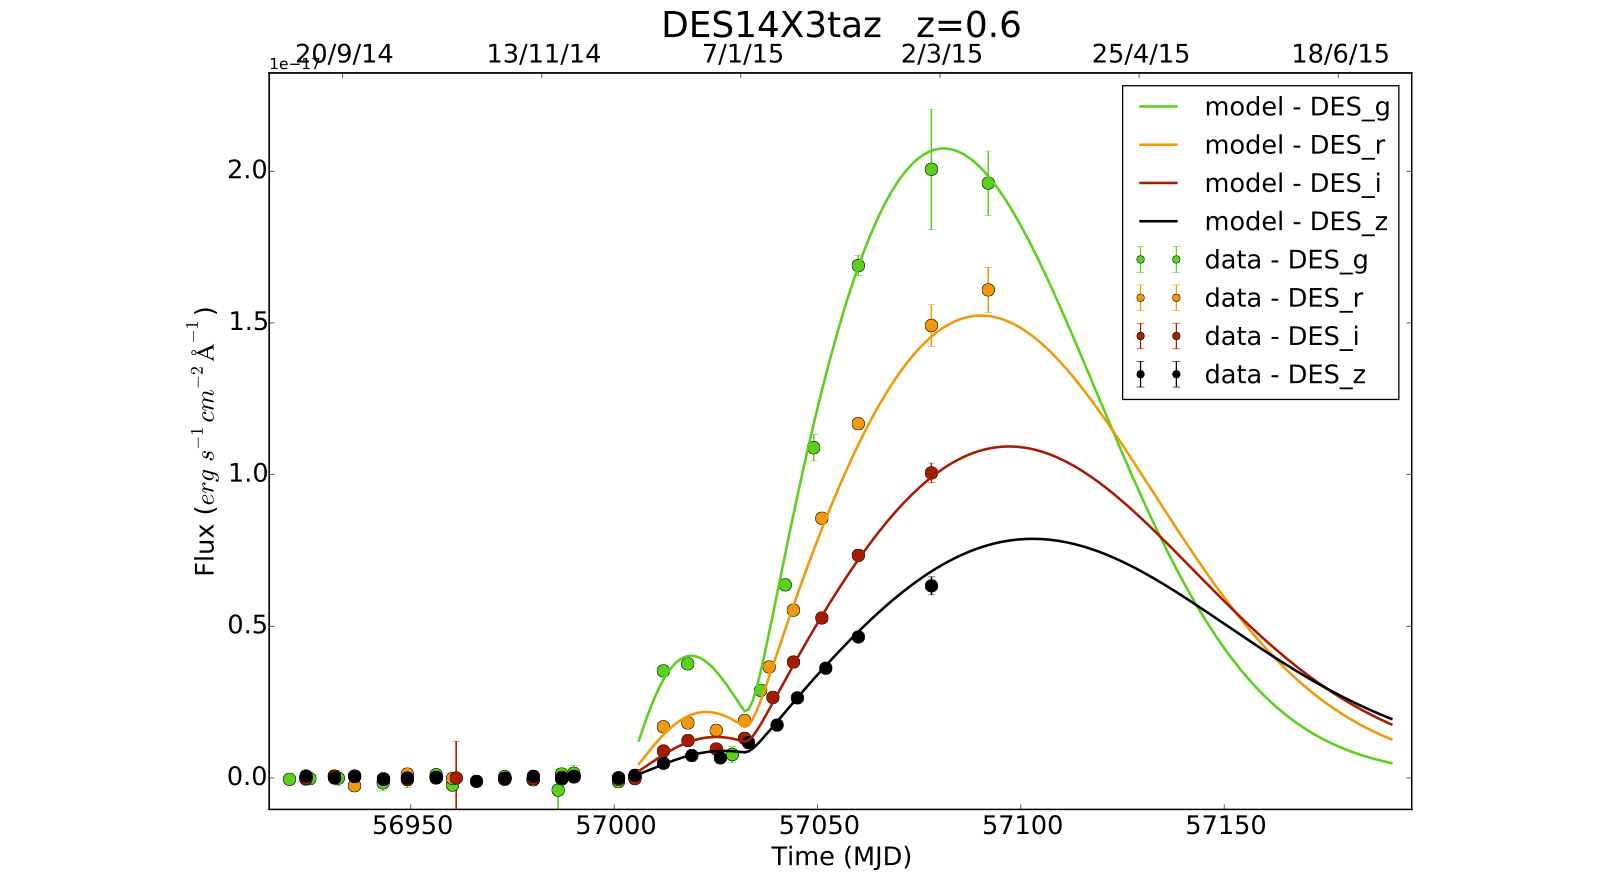
\includegraphics[width=\textwidth]{Figures/Chapter4/DES14X3taz}
  \caption{SLSN DES14X3taz fit with the combined Magnetar and \citet{Piro2015} models. Combining the models breaks the degeneracy between the kinetic energy of the SN explosion energy and the ejecta mass allowing for a direct measurements of these values.}
  \label{fig:PiroMagnetar}
\end{figure}

\paragraph{R$_0~>$ 0}
\label{par:R0nonzero}
While it is widely accepted that the birth and a spin-down of a magnetar is the most likely progenitor of SLSN, the exact process through which the high-energy radiation produced by the magnetic breaking is transported into the outer shells of the ejecta is not yet understood. If the injection of energy does not closely coincide with the time of the explosion of the progenitor star, the SN could go through a "grey" phase, powered only by the explosion energy of the SN, followed by a rapid rebrightening at the point of the spin-down energy injection. In several cases, including PS1-11ap and DES14X3taz (where we exclude the pre-peak bump data), the magnetar model does not fit the earliest stages of the light curve correctly.

In order to investigate this delay, I have introduced a non-zero initial radius of the progenitor. While the radius of the progenitor star is never zero, it is usually negligible in comparison with the expansion velocity of the ejecta. However, in the case of DES14X3taz and PS1-11ap, I found initial radii consistent with ejecta that underwent an expansion, at a constant velocity, for 17 and 9 days respectively. PS1-11ap has no observations prior to its first detections making it impossible to determine if the object was associated with a pre-peak event. As shown in \fref{fig:PS1-11apR0}, this technique, can provide insight into the mechanism behind the magnetar energy injection even in the absence of the earliest and pre-explosion epochs.

\begin{figure}
  \centering
  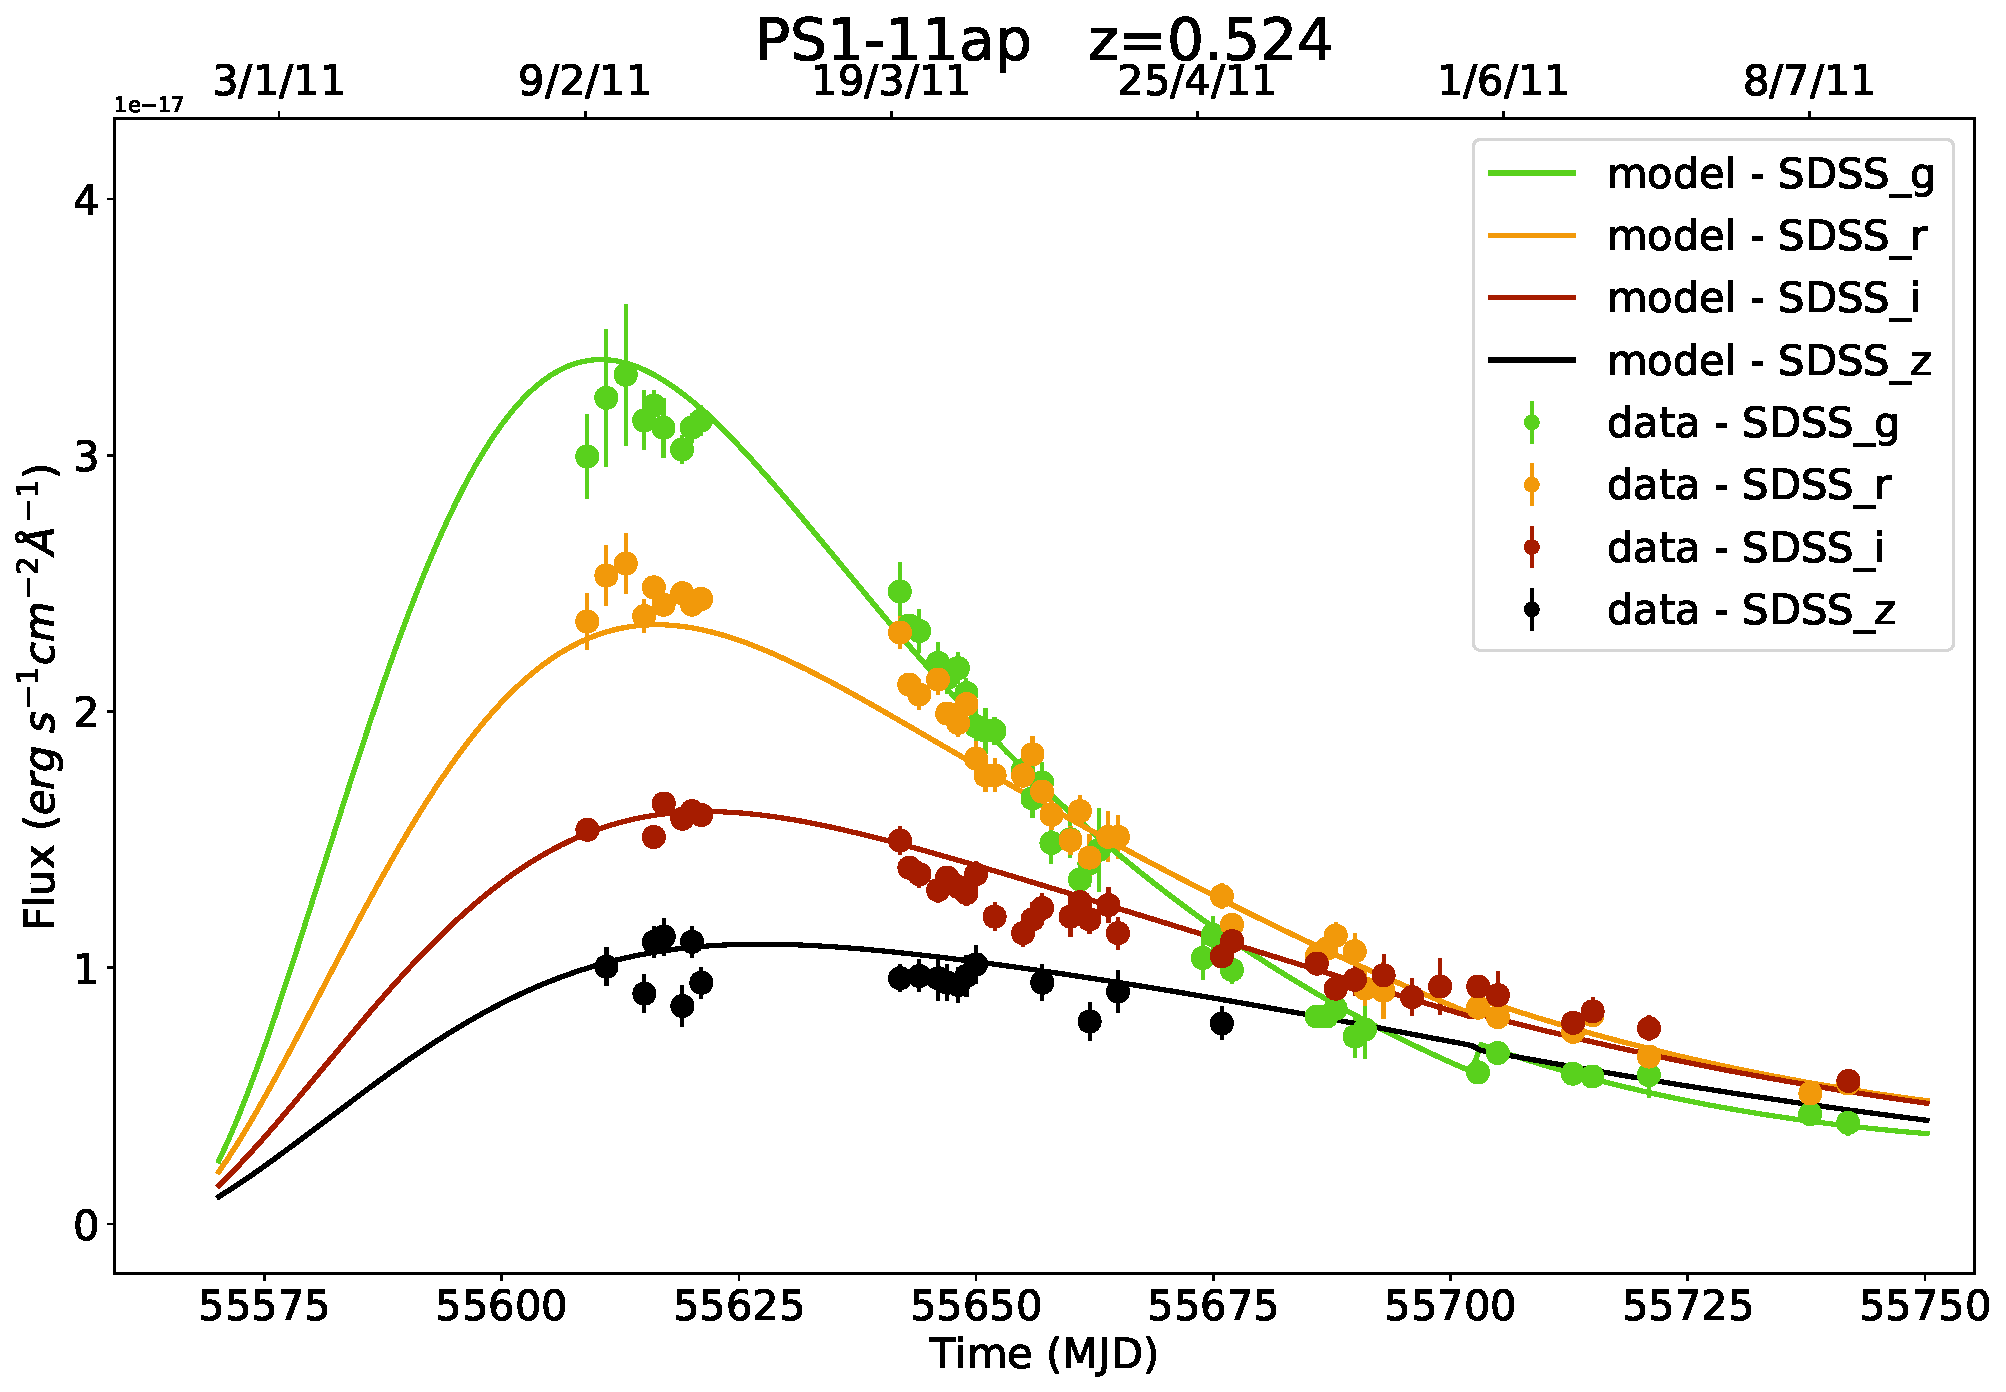
\includegraphics[width=\textwidth]{Figures/Chapter4/PS1-11ap}
  \caption{The magnetar model fit to a SLSN, PS1-11ap. The model does not assume the initial radius of the SN to be zero at the onset of the spin down of the Magnetar, instead it is fitted as a free parameter. The value for $R_0$ found for PS1-11ap is consistent with a ejecta that has undergone expansion for 9 days prior to the onset of the Magnetar}
  \label{fig:PS1-11apR0}
\end{figure}

\paragraph{Nickel decay}
Another interesting questions that we were able to investigate using \textsc{SLAP} is the contribution from the radioactive decay of Ni56 and Co56 as an additional energy source powering the ejecta. I have introduced this to investigate a potential mechanism powering the peculiar, flat evolution of DES13S2cmm. In this model, I add the contribution from the decay of these radioactive elements into the bolometric luminosity of the SN and do not introduce any other modification to the model. While we find that the radioactive decay alone cannot account for the evolution of DES13S2cmm, this test demonstrated the ease with which we are able to modify our models to test new assumptions. The evolution of DES13S2cmm is further investigated in Angus (in prep).

\subsubsection{Maximum Likelihood methods}
The success of \textsc{SLAP} in fitting SLSNe cannot be attributed only to our work on the models but, perhaps in the largest part, to the optimisations applied to the fitting routines. One of the main goals for \textsc{SLAP} was a full autonomation of the fitting process, without the need for manual fine-tuning of any input parameters. This is crucial for performing fits on large datasets, containing thousands of objects where only a small fraction are likely to be good matches to the model. Furthermore, we do not wish to introduce any human biases to the fitting procedure, particularly in the case of the ML training sample as the techniques used by us are sensitive enough to recover such biases over the true trends in the data.

In the early stages of the project, we have explored fitting the model using the Maximum Likelihood Estimate (MLE) method. This approach is based on maximising the Likelihood function which, in the frequentist approach, describes the probability of the observed data originating from the underlying model. As the uncertainties in our observations are normally distributed I use the Least Squares (LS) regression analysis which is a special case of MLE. In LS fitting, we minimise the residual, defined as the uncertainty weighted difference between the data and a model, using the $\chi^{2}$ test as a metric for defining the goodness-of-fit:
\begin{equation}
  \chi^2 = \sum\limits_i^N \left( \frac{O_i - m_i}{\sigma_i} \right)^2
\end{equation}

\paragraph{MPFIT} \label{sec:MPFIT}
The MLE fitting approach was implemented in \textsc{SLAP} using \textsc{MPFIT} \citep{ Markwardt2008}, based on \textsc{Fortran}'s package \textsc{MINPACK} \citep{More1980}. \textsc{MPFIT} is an implementation of the Levenberg–Marquardt non-linear LS fitting algorithm \citep{Levenberg1944,Marquardt1963}. This is a popular and highly optimised example of the class of iterative, gradient descent algorithms that work by traversing the likelihood function, moving in the direction of lower $\chi^2$ (i.e. higher likelihood). The algorithms use a gradient (either analytical or numerical) of the likelihood function to inform the direction and size of a jump taken at each iteration. In the Levenberg–Marquardt algorithm a damping coefficient is introduced decreasing the number of steps taken by the algorithm before converging on a minimum.

While \textsc{MPFIT} was very promising during our testing, we discovered that the quality of our fits strongly dependant on the choice of the initial parameter guesses. This is a common issue amongst all gradient descent algorithms informed only by the gradient at the measured point. This leads to them finding the local likelihood maximum, nearest to the initial parameter guess instead of the global value. This contradicted one of our strongest demands for the package, as \textsc{SLAP} would require manual modification for the initial parameter guesses, making it impossible to use with a large number of objects.

\subsubsection{Bayesian Inference}
While a number of global optimisation approaches have been trialled, we realised that the complexity and degeneracies of the magnetar model require a fully Bayesian treatment in order to efficiently find the global minimum (or Maximum Likelihood) of the model. Bayesian Inference is a technique based on the Bayesian approach to probability, derived from Bayes' Theorem which states that for a set of model parameters $\mathbf{\theta}$ and data $\mathbf{D}$:

\begin{equation}
  P(\mathbf{\theta}|\mathbf{D}) = \frac{P(\mathbf{\theta}) P(\mathbf{D}|\mathbf{\theta})}{P(\mathbf{D})}
\end{equation}

\noindent where $P(\mathbf{\theta}|\mathbf{D})$ is the Posterior Probability, $P(\mathbf{\theta})$ denotes the Prior Probability, $P(\mathbf{D}|\mathbf{\theta})$ defines the Likelihood and finally, $P(\mathbf{D})$ is the model Evidence.

The Posterior Probability describes the probability of the model $\mathbf{\theta}$ given the observed data $\mathbf{D}$. The biggest difference between the frequentist and Bayesian view of probability is the inclusion of the Prior Probability which describes our believe in the model before we make the observations $\textbf{D}$. The Likelihood function here is analogous to the Likelihood function used in MLE. In fact, in the special case where the Prior distribution is uninformative (i.e flat), Bayesian Inference is equivalent to MLE and would yield the same result. The Evidence, $P(\mathbf{D})$, acts as a normalisation constant and is only used in comparing distinct models and not in determining their "best-fit" parameters. $P(\mathbf{D})$ is usually very difficult to compute as it requires the Likelihood function to be integrated over the entire parameter space. The following paragraphs describe the methods I used for computing the Posterior Probability distribution as well as estimate the model Evidence.

\paragraph{MCMC}
Markov chain Monte Carlo (MCMC) is an extremely popular and widely used set of techniques for estimating the Posterior distribution. One of its simplest implementations, the Metropolis-Hasting algorithm, iteratively samples the Posterior distribution by drawing a new point from the normal distribution centred at the previous parameter and accepts it if the value has a higher probability. However, what differentiates the MCMC approach from MLE techniques is that a sample can also be accepted if it has a lower probability that the previous point in the chain. The acceptance ratio here is defined as the ratio of the new probability to that of the previous iteration. This allows the 'walker' to sample the entire Posterior Probability distribution provided that the chain a sufficiently long.

In this thesis, I have tested both a custom MCMC implementation as well as the popular and heavily optimised, multithreaded package, \textsc{Emcee} \citep{Foreman-Mackey2012}. While both approaches can estimate the Posterior distributions as well as the best-fit parameters with no external input or hyperparameter fine-tuning, their performance based on a need to evaluate millions of models to provide a full sampling of the Posterior distribution, was however very poor. A light curve fit would often require in excess of 8 CPU hours, despite the heavy optimisations of the model.

\paragraph{\textsc{MultiNest}}
A recently developed technique for approximating the Posterior Probability distribution, showing a great improvement in efficiency is Nested Sampling \citep{Skilling2006}. Here, the Posterior distribution is calculated as a by-product of the model Evidence evaluation. While this is usually a very computationally expensive calculation, Nested Sampling uses the properties and relationship between the likelihood and the prior to reducing the multi-dimensional integral into a single dimension, which is simpler to evaluate. The algorithm populates the prior with a relatively small (I used 2000) 'live' points which calculate the Likelihood. The point with the lowest Likelihood is replaced by a new point, geometrically closer to the point of highest Likelihood. The new point is accepted if its Likelihood is higher than the point it originally replaced. Nested sampling provides a near 1000-fold efficiency improvement over the common MCMC methods. This makes the approach of using Nested Sampling sufficiently fast and robust to satisfy the design requirements of \textsc{SLAP}.

In this thesis, I use \textsc{MultiNest} \citep{Feroz2009,Feroz2011,Feroz2013}, a Fortran based implementation of the Nested Sampling algorithm. This is one of the most popular implementations of the technique. It is robust and thoroughly tested in a number of cosmological studies using the CosmoMC package \citep{Lewis2002}, making it the perfect package for us. One of the greatest advantages of \textsc{MultiNest} is its operation in a multi-modal mode where the algorithm returns not only the Maximum-a-Posteriori (MAP) parameters but also positions of other, local, maxima. [SHOULD I PUT AN EXAMPLE CHAIN/CORNER PLOT HERE?]

\subsubsection{pyMagnetar}
While SLAP was very heavily used throughout this thesis as a tool for modelling SLSNe, putting an emphasis on the optimisations involving model fitting, I have also used it as a tool for building synthetic catalogues of SLSNe. While this was directly possible using the C++ frontend, it is difficult and inefficient to interface the code with the majority of modern astronomy pipelines which are most commonly written in \textsc{Python}. Using the \textsc{Cython} language, I have created a higher level interface to the code, \textsc{pyMagnetar}. I have also implemented a further level of optimisation by fine-tuning the code to work with a single set of photometric bands (e.g DES or SNLS). As the code no longer needed to consider any arbitrary filters, its performance has increased considerably.

\section{Modeling CCSN}
The recent years saw an increased interest in modelling of CCSN driven by the development of large area surveys such as LSST and ZTF. The predicted numbers of transient discoveries exceed our ability to classify the SNe using the conventional, manual techniques. The modern approach using machine learning classifiers require a large number of training samples, distributed evenly amongst all subclasses of SNe. The number of real objects observed to date is not sufficient to act as a training sample alone. It must, therefore, be supplemented by an artificial or augmented sample of SNe, generated from a set of template SN.

Amongst a number of past CCSN templates \citep{Schlegel1995,Nugent2006}, \citet{Kessler2009} has been the most commonly used tool for creating artificial samples of SN in recent years. Packaged as part of the \textsc{SNANA} suite of analysis and simulation tools, it is widely used in a number of leading surveys including SDSS, DES and PS1 as well as ML studies of SNe \citep{Kessler2010,Lochner2016}. Despite its popularity, \textsc{SNANA}'s templates have a number of drawbacks \citep{Kessler2010}. In \textsc{SNANA} a single spectroscopic template per SN subclass \citep[Taken from]{Nugent2006} is warped to match the photometry of a number of SN light curves observed by SDSS, SNLS and CSP. While generating 43 templates for CCSN (overall subclasses, as per the latest release of \textsc{SNANA} \citep{Jones2016}), they do not account for the diversity in the SEDs of CCSN nor their evolution. Furthermore, the pseudo-templates, generated from a single spectroscopic master-template, have a narrow wavelength coverage not extending considerably below the rest-frame SDSS \textit{u}-band filter and, in the majority of cases, above the SDSS \textit{i}-band.

In order to create a modern set of templates, suitable for ML studies of SNe, we present a new set of tools which move away from the approach of using the master templates found in \citet{Nugent2006}. We use all available, high quality photometric and spectroscopic data for CCSN found in the literature in order to create templates that are not correlated with each other. We also use auxiliary UV data to extend the SED to lower wavelengths allowing, for the first time, to simulate these objects in all bands at all redshifts where the SNe are detectable in DES and LSST.

In this section, I describe the main design choices behind both CoCo and pyCoCo, the packages developed to create spectroscopic templates of CCSNe as well as simulate them in a number of surveys. I discuss the models used in modelling the CCSN light curves and those undertaken to create their spectroscopic templates. I then describe the steps taken to extend out spectroscopic templates into both the UV and IR parts of the SED, not covered by the observed spectra.

\subsection{\textsc{CoCo}}
At a basic level, the packages I developed as tools for simulating CCSN are very similar to \textsc{SLAP}, used in the modelling SLSN. Its performance, similarly to \textsc{SLAP}, was a critical part of the code design as we aim to simulate millions of light curves in LSST and DES. This lead to our decision to, again, follow the principle of developing the core of the package in \textsc{C++} and using \textsc{Cython} to create a \textsc{Python} front-end interface. I will follow our internal naming for the packages and refer to the backend packages, developed in \textsc{C++}, as \textsc{CoCo} and the \textsc{Python} front-end wrapper as \text{pyCoCo}.

\textsc{CoCo} consists of four core packages, \textsc{LCFit} used to fit the SN light curves with a number of models, \textsc{SpecFit} used to match the observed spectra to the photometry, \textsc{SpecPhase} which assigns the phase to each spectrum and corrects them to a common redshift and finally \textsc{LCSim} which can be used to simulated SN based on the outputs of the previous three packages. In the following subsections, I will describe these packages as well as the models, decisions and assumptions we made that led to the final product.

\subsubsection{\textsc{LCFit}} \label{sec:LCFit}
The process of creating the spectroscopic templates of CCSN start by fitting the observed light curves for the SNe with an analytical model able of describing their morphology as well as reliably extrapolating them. This step is required in order to later flux calibrate the observed spectra to match the observed photometry. The interpolation allows us to calibrate the spectra on epoch where there was no photometric data point available. While a non-parametric approach could be used such as Spline Interpolation or Gaussian Process Regression, we required an ability to extrapolate the light curve fits beyond the range of the observed point for the cases where the spectroscopic follow-up either exceeded that of the photometry or, in even rarer cases, preceded it in time.

At this phase of the procedure, the models are fitted using the \textsc{MultiNest} fitting routine. We followed a similar method to that used in \textsc{SLAP}, giving us the state of the art fitting accuracy and reliability. The photometry is fitted independently for each band. Thanks to the use of a Bayesian fitting routine, the resulting fit gives us the curve of best fit as well as a confidence region for the model. For technical reasons we do not store the best-fit parameters, instead, we store a dense sample curve of best fit and its corresponding region of confidence.

In this thesis, I have trialled and implemented a number of models found in the literature as tools for fitting the light curves of CCSN. In the following sections, I give their brief overview and discuss their benefits and drawbacks in the context of this project. The comparison of the models used in this thesis for an example SNXXXXXX is shown in \fref{fig:CCSNModelFits}.

\paragraph{Bazin09}
The simplest, yet the most versatile, model for describing CCSN can be found in \citet{Bazin2009} (Bazin09 from here). This simple model is a combination of a logistic function which describes the rise of the SN and an exponential decay which matches the decline of the light curve (\eref{eq:Bazin09}). This model was successfully used to photometrically identify CCSN-like events in the SNLS. While the simplicity of the model means that it is not able to fully describe the behaviours of all SNIb/c, it provides a good match to those dominated by the radioactive decay of Nickel56 as their power source. We have found it to be very powerful in the cases where the observed light curve was sparsely sampled as, even in the most difficult cases, the model can produce a well-constrained solution that matched the expected features of a SN.

\begin{equation}
\label{eq:Bazin09}
  F(t) = A \frac{e^{-\frac{t - t_{max}}{\tau_{fall}}}} {1 + e^{\frac{t - t_{max}}{\tau_{rise}}}}
\end{equation}

\paragraph{Kessler10}
A more complex version of the model used in \citet{Bazin2009} was used in \citet{Kessler2010} (Kessler10) as a base for their work on creating a photometric sample of CCSN for the use in the Supernova Photometric Classification Challenge. While the model parameterises SN using an underlying exponential decay and rise, it additionally provides the ability for the model to account for a secondary maximum often observed by SNIa. As CCSN rarely show signs of a secondary maximum, the extra degrees of freedom often improve the early fits around the early rise time phases of the SN where there are other mechanisms in action (e.g shock breakout, Hydrogen recombination etc.) that inject additional energy into the early light curves.

One drawback of this model and the reason why, on average, we have found it to not improve the quality of our fitting is the common timescale behind the decay of the primary and secondary maxima. This does not correspond to the observed behaviour in CCSN where the power sources are not physically linked and therefore act on different dynamic timescales.

\begin{equation}
  F(t) = A \times [1 + a_1(t - {t_0}) + a_2(t - {t_0})] \times \frac{e^{-\frac{t - t_{0}}{\tau_{fall}}}} {1 + e^{\frac{t - t_{max}}{\tau_{rise}}}}
\end{equation}

\paragraph{Karpenka12}
\citet{Karpenka2012} (Karpenka12) further improves on the model found in Kessler10 by decoupling the onset of the primary and secondary peak. While retaining the same number of free parameters as Kessler10, the improvements in the fitting quality are considerable for the SN\,Ib/c with a more complex morphology.

\begin{equation}
  F(t) = A \times [1 + B(t - {t_1})^2] \times \frac{e^{-\frac{t - t_{0}}{\tau_{fall}}}} {1 + e^{\frac{t - t_{max}}{\tau_{rise}}}}
\end{equation}

This model was successfully used in a project involving SN photometric classification using basic Neural Networks \citep{Karpenka2012}, demonstrating that it is a suitable model for our use.

\paragraph{Firth18}
Finally, we considered a new model introduced in Firth et al. (in prep; Firth18), based on the Karpenka12 model with an additional, fully independent of other properties, logistic decay term which can be used to model the shock breakout phase observed in some SN.

\begin{equation}
  F(t) = A \times [1 + B(t - {t_1})^2] \times \frac{e^{-\frac{t - t_{0}}{\tau_{fall}}}} {1 + e^{\frac{t - t_{max}}{\tau_{rise}}}} \frac{1}{1 + e^{\frac{t - t_{pre}}{\tau_{pre}}}}
\end{equation}

The additional term introduces in this model means renders it only compatible with light curves containing a large number of data point where this pre-peak event will be constrained to null in case of a lack of an observed shock breakout event, or those with a well-defined event. In other cases, the extra degrees of freedom simply act as an additional degeneracy in the modelling and often results in a lower quality fit than using a more basic model.

\begin{figure}
  \centering
  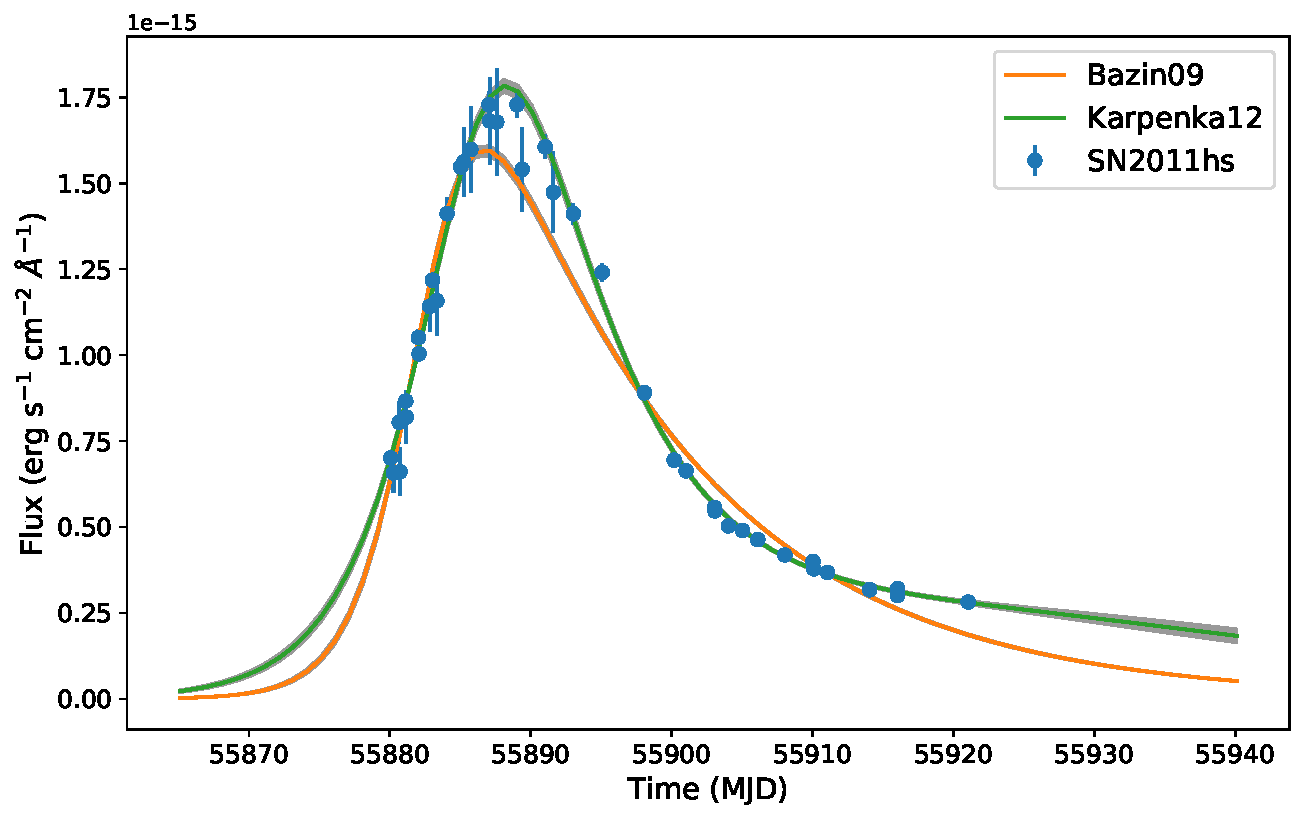
\includegraphics[width=\textwidth]{Figures/Chapter4/CCModels}
  \caption{The light curve of SN2011hs, a SNII, fit with the Bazin09 and Karpenka12 models for comparison. Both models are based on the same exponetial decline and logistic rise function. However, Karpenka12 adds and additional term that allows for the change of slope in the light curve decline as observed in this SN}
  \label{fig:CCSNModelFits}
\end{figure}

\subsubsection{\textsc{SpecFit}}
One of the most crucial parts of our procedure for generating templates of CCSN is the matching of the observed spectra to the flux to the photometry. Due to the complexity of spectral data reduction and flux calibration, the uncertainties associated with their measurements can be high, and more problematically, wavelength dependent. The accuracy of the spectral flux is particularly important in the case of high precision surveys including PS1, DES and LSST where the photometric accuracy is particularly high, exposing the uncertainties from other sources such as SN simulations \citep{Jones2016}. The process used to correct the flux calibration, referred to as spectral 'mangling', adjusts the spectrum such that the synthetic flux measured by passing the spectrum through filter bandpass response functions matches the observed photometry. I have encapsulated this in the \textsc{SpecFit} package.

In order to adjust the spectrum, a spline is applied to it, designed in a way to smoothly correct the spectra, as shown in \fref{fig:SpecMangling}. A spline is a smooth, continuous function defined using a number of control points; a position and amplitude. The wavelength at which we place the control points matches that of the central wavelength of the filters while the amplitude is determined using a numerical minimisation routine. We again use \textsc{MultiNest} as our fitting tool. The choice of the endpoints of the spline is important. In this code, I have placed them at 100\AA outside of the wavelength range of the mangled spectrum. The amplitude of these points is not subject to the fitting, instead, they are determined by extrapolating two most extreme points on either side of the spectrum using a straight line.

\begin{figure}
  % \includegraphics{/path/to/figure}
  \caption{\textit{top}: An example spectrum of SNxxxxx before mangling  }
  \label{fig:SpecMangling}
\end{figure}

While developing the mangling code, we discovered several issues which had to be addressed before reliable results could be obtained. One of the major issues arose due to control points of the splines positioned to close to each other, causing the interpolated function to behave erratically and far from the expected. We have traced this to using filters which are derivatives of each other, such as Johnson's R and SDSS-\textit{r}, that only vary in central wavelength by $\sim$50\AA. This would not result in a problem if the control points were already correctly calibrated but, due to the nature of the fitting process, the points were fit independently causing large, non-linear degeneracies that cannot be controlled even using routines as powerful as \textsc{MultiNest}. We were, therefore, forced to remove the overlapping spectra from the mangling. As we focused on preserving the maximum information in the bluer part of the SED, we have retained the band with a lower central wavelength.

Furthermore, we have found that the mangling is not reliable when less than three bands are used to set the control points. This is caused by the endpoints being extrapolated using the previous two points. Spectra that overlapped with only two distinct bands could therefore not be used as the control points used for the extrapolation were the same for the upper and lower limits, causing degeneracies that were difficult to handle with even sophisticated fitting routines. As a final product, \textsc{SpecFit} saves the flux calibrated spectrum in the ASCII format, scaled to the observed photometry at the original redshift of the SN.

\subsubsection{\textsc{SpecPhase}}
A major difference between my approach to fitting the SLSNe and CCSN is the treatment of their explosion date (or the start date of the simulation). In the case of SLSNe, we have a well-defined explosion date, set as a free parameter in our model, prior to which we can assume the flux to be null. In the case of the models used in \sref{sec:LCFit}, their rise is not abrupt but following a logistic function which only tends towards zero at negative infinity, making it impossible to define the explosion date without any adding assumptions.

We must, therefore, define the time at which we insert the light curve in our simulations using a different system. In this case, we use the time of the maximum light of the SN as the point of reference, measured in the rest-frame V-band. The phase is determined in the following way; the spectra are shifted to z=0 (rest-frame). Using the distance moduli for the host galaxies obtained from the NED archives \citep{Tully1988}. I scale the flux for each spectrum to give their apparent flux at 10pc (e.g the absolute magnitude). I then synthesis a V-band light curve from the spectral time series and fit it using the same approach as in \sref{sec:LCFit}. The peak is determined numerically as the maximum of the light curve fit. Finally, the package returns a list containing the phases, relative to peak, for each spectrum per object as well as a spectral time series normalised to z=0 and absolute magnitude of the SN.

\subsubsection{\textsc{LCSim}}
Following the previous steps, we can obtain a set of spectral templates that can now be used to generate a new sample of synthetic SN light curves. This step is based on the same concept as \textsc{SpecPhase}, used to determine the phases of the template spectra. The template spectra are shifted to the required redshift and corrected for the distance modulus. The spectra are also corrected for the host galaxy extinction, before they are redshifted, as well as the milky way extinction once at the observed redshift. Synthetic photometry is them generated for the requested bands before a light curve model is fit to it, allowing for simulated photometry points to be generated at an arbitrary phase.

\textsc{LCSim} is the only package as part of \textsc{CoCo} that does not rely on \textsc{MultiNest} as a minimisations tool. While it would have been optimal from the accuracy and robustness point of view to use it, we have found that its performance was insufficient in order to simulate millions of CCSN, as required. After discovering issues with numerical instabilities in \textsc{MPFIT} (used in \sref{sec:MPFIT}) when computing the derivative of our residual function, we have decided to use a more modern package, \textsc{Minuit2} \citep{James1975}. Designed by CERN and heavily used within the ROOT library \citep{Brun1997}, \textsc{Minuit2} utilises more modern numerical libraries which helps it to handle numerical uncertainties better than its \textsc{Fortran} derived predecessors. \textsc{Minuit2} implements a number of algorithms derived from the broader gradient descend family. In \textsc{LCSim} we use \textsc{migrad} which is the default minimiser in the package and is based on the same concept as the Levenberg-Marquardt algorithm used in \textsc{MPFIT}.

\subsection{pyCoCo}
Following the same design pattern as in \textsc{SLAP}, I have created a \textsc{Python} interface for the \textsc{LCSim} package using the \textsc{Cython} intermediate language. The ability to interface the code with \textsc{Python} allowed me to manipulate the simulated light curves directly in the memory without the need to create a time and memory consuming intermediate output, significantly reducing the overheads in the simulation. This also simplified the process of storing the final simulations by interfacing the output directly with a \textsc{PostgreSQL} database.

As the package was always intended for a wider audience, not limited purely to this project, \textsc{pyCoCo} forms a simpler and more approachable interface to \textsc{CoCo}. Furthermore, Firth et al. (in prep) have built a large suite of wrappers and tutorials for template generation which compliment \textsc{pyCoCo} and allow for the whole procedure to be performed directly from \textsc{Python}.

\subsection{SN\,Ib/c SED UV Extensions}
SN\,Ib/c were the main focus of \textsc{CoCo}. Their simulations are some of the most desired amongst various classes of SN as they are the main source of contamination in the samples of SN\,Ia due to the similarities in the physics that powers their luminosity. SN\,Ib/c are, however, relatively rare in comparison to SN\,Ia or even hydrogen-rich SN.   Firth et al. (in prep) collected a sample of `good' SN\,Ib/c lightcurves and their respective spectra from the literature. 29 SNe were part of the initial sample before extra quality cuts were applied. The final sample included 17 SNe that were used to generate the templates.

As could be expected from such a diverse sample of objects, a large number of the spectra do not have a very good wavelength coverage, often not exceeding the range of 4000-7000\AA. On a contrary, the light curves for almost all SN in the sample include the minimum of BVR bands with a number of objects including both redder and bluer bands. It was, therefore, possible to use the extra light curve information as a base upon which we can extend the spectroscopic templates of the SNe. Red extensions were required in order to simulate the low redshift SN in the reddest bands (e.g. DES \textit{z}-band). These extensions were performed as part of Firth et al. (in prep) and used a black body to extend the spectra up to 10500\AA. The flux was then corrected to the photometry by again passing the spectral time series through \textsc{SpecFit}.

In contrast with the red extensions, we could not rely on the observed photometry for the blue wavelength extensions. As we aim to simulate SN\,Ib/c to redshifts of up to z$\approx$0.8 in the DES deep-fields, we require the templates to extend to $\sim$2000\AA in order to overlap with the observer-frame \textit{g}-band at that redshift. The required region of the light curve most closely matches that of the Swift-UVOT UVW1 filter \citep{Roming2005}. The Swift satellite launched in late 2004 as a rapid response Gamma-Ray Burst (GRB) detector. Since then, it observed a number of SNIb/c, giving us a glimpse at their UV light curves. The data, however, is not present for all objects rising a need to approximate the behaviour for the objects with no UV data.

Using the data collected by the Open Supernova Catalogue \citep[OSC;]{Guillochon2017}, I have created a subsample of our template SNe with available UV data. Amongst these, a large number of objects only included the very earliest epochs likely triggered as a follow-up based on the x-ray detections of the object. A number of these objects, however, did later received an extended follow-up campaign, giving us light curve information past maximum light. For these objects, I have performed light curve interpolating using Gaussian Process Regression (\cref{sec:GP}). This allowed me to compare the UVW1 light curve to the V-band, as shown in figure \fref{fig:VvsUVW1}, showing that during the main phase of the SN (excluding the shock breakout), the UWV1 and V band light curves followed a very similar evolution. The UVW1 were found to be 2.5 magnitude dimmer (10 times dimmer in flux). I, therefore, use this property to create artificial UVW1 light curves by offsetting the V-band light curve by 2.5 magnitudes in flux and retaining its overall evolution.

\begin{figure}
  % \includegraphics{/path/to/figure}
  \caption{The ratio between the UVW1 and V band filters plotted for a number of stipped envelope SNe.}
  \label{fig:VvsUVW1}
\end{figure}

Using the extended light curve coverage we can extend the spectra following a similar process to that used for IR extensions. As there is little information about the UV spectral evolution of CCSN, I follow the same technique as Firth et al. (in prep) by using a black body to extend the SEDs. We again pass the extended spectrum through \textsc{SpecFit}, matching the spectrum to the synthetic UVW1 photometry.

\subsection{SN\,II with CoCo}
The aim of Firth et al. (in prep) was predominantly to generate a sample of SN\,Ib/c to aid the classification studies of SN\,Ia for cosmological uses. While our packages were developed to tackle SN\,II in a similar analysis, this was never attempted as part of Firth et al. (in prep) and instead was performed only as part of this thesis. In large, I have followed the same methodology with several steps that were optimised to better suit SN\,II or improvements based on the lessons we have learned in Firth et al. (in prep). I will also use this opportunity to describe the steps taken to produce the sample of spectral templates in a project similar, but performed independently, of Firth et al. (in prep).

All data in this project was obtained using the OSC repository. The data was collected for objects matching the hydrogen-rich SN subclasses including SNII, SNIIP, SNIIL, SNIIn, SNIIb and SN1987A-like. Only the objects with a light curve coverage including the pre-peak and post-peak data, as well as a relatively dense spectral coverage,ß        covering the same regions as the light curve, were included in our sample. I have used the toolkits developed in Firth et al. (in prep) to nightly average any spectra that were taken in rapid succession. I have also removed the regions of each spectrum where no SN light was detected or the S/N was too low to confidently recover the underlying morphology of the SED.

In the next step, I removed all spectra with a coverage shorter than two photometric bands. I also removed the spectra that did not overlap with the V-band. Following these clearing stages, I again removed the objects that now no longer satisfy the coverage required for our analysis. The above steps retained a sample of 11 objects with sufficient quality of the use as templates for CCSNe.

The light curves for all retained objects were fit with all models described in \sref{sec:LCFit}. While, due to the increased number of degrees of freedom, the more complex models such as Karpenka12 and Firth18 are able to fit the data more precisely, they are unable to constrain light curves will a small number of data epochs. In the process of simulating the light curves, we fit the models to photometry synthesised from the spectra which are sparse for most objects in our sample. Instead of using the more complex models, I fit all SN in the sample with the most basic Bazin09 model. Despite its lack of complexity, it produced a good fit to all light curves in our sample. I note here that this was not the expected result. SNIIP are associated with a light curve plateau phase which could not be accounted for in this model. However, none of the objects that observe this behaviour had sufficient spectral coverage to pass the previous quality cut. This is not an optimal scenario as a whole class of objects are, seemingly, excluded from the sample. The plateau is, however, more prominent in the redder bands and therefore does not appear as a strong feature in the rest-frame blue bands that form the majority of the observed SED at high redshift where we simulate the majority of our SNe.

A major difference between the work undergone on SN\,II in this thesis and that on SN\,Ib/c in Firth et al. (in prep) is the treatment of the spectra before \textsc{SpecFit} is used to apply the mangling step. In Firth et al. (in prep) we excluded all spectra that did not have a sufficient wavelength coverage to successfully undergo mangling. We found that spectra with a coverage shorter than three filters were not able to constrain the spline function. In many cases, the spectra were only short of few hundred Angstrom, most often in the red part of the spectrum. Instead of removing such objects, I used linear extrapolation from the final 100\AA of the observed spectra to the wavelength required in order to complete the coverage of the third filter. This helped to retain a much larger number of spectra, in some cases saving the object from being removed from the sample under our quality cuts.

Another major difference between the projects is the approach to extending the light curves in both the IR and UV regimes. In the IR, I found that a number of SN\,II spectra would fail to fit a black body function. At this stage, such objects were removed from the Firth et al. (in prep) sample. To retain the maximum number of objects I have instead fit the objects using an exponential decline function. As a simple numerical form, this function can correctly fit all objects. It is not necessary for this function to physically correspond to the expected SED as the mangling step corrects this later.

The method used for the UV extensions were also modified. The UV data for the SN\,II was very limited. It shows that these objects raise as very UV bright but rapidly evolve in colour, quickly losing all of their UV flux. This meant that the same methodology of creating an artificial UVW1 band by scaling any of the optical bands. The number of objects with a sufficient UV coverage was also insufficient to obtain a relationship between the UV and optical evolution of the SNe. As an approximate solution, I have extended the spectra of SN\,II by fitting their SEDs with a black body model and did not follow it with a mangling step. In figure \fref{fig:SNIIbbExtension} I compare the evolution of the modified spectra to an example light curve of SNXXXXX, showing that this is a good, first-order approximation.

\begin{figure}
  % \includegraphics{/path/to/figure}
  \caption{}
  \label{fig:SNIIbbExtension}
\end{figure}

\section{Gaussian Processing} \label{sec:GP}
One of the biggest obstacles, and perhaps the main reason, behind SN classification, still relying on non-ML approaches is the irregular nature of the observing cadences. As a broad simplification, ML techniques rely on recognising repeating sequences or patterns. In order to recognise patterns independently of their position along the time series, they must be uniformly sampled. Without this, any classifiers would bias the result towards a preferential explosion time. Moreover, even in cases where we would be willing to accept this drawback, there is a limited number of algorithms that are designed to work with unevenly sampled data.

Previous SN studies using ML approaches used physically motivated features extracted from light curve model fits. In the most complete study of this kind to date, \citet{Lochner2016} fit the SALT2 SN\,Ia model to a number of SN classes and used these properties to classify the SNe. I am reluctant to follow a similar path as I feel that this approach was only successful because it focused on the classification of SNe with a similar morphology (SN\,Ia and SNIb/c), motivated by the physics of their central engines. The SALT2 model is incapable of reproducing the light curves of SLSN and other peculiar transients. This would result in a classification very strongly dependant on the quality of the light curves e.i. SALT2 could produce a SNIa-like light curve if fit to very low S/N data based on its priors alone.

My aim in this section is to develop a method for interpolating SN light curves using a non-parametric approach in order to enable the classification of SN using ML models that do not rely on explicit feature extraction. Amongst a number of approaches that I have considered in this thesis, Gaussian Processes introduces an extremely powerful and robust way of modelling the light curves.

\subsection{Theory}
Gaussian Process (GP) \citep{Rasmussen2006} is defined as a set of normally distributed random variables, (x, y), where any subset of them can be drawn from a joint Multivariate Gaussian Distribution, $\mathcal{N}$, defined using the mean of the data, $\bar{y}$, and a covariance function, $K = k(x, x'|\mathbf{\theta})$. The process of interpolating data using GPs is referred to as Gaussian Process Regression (GPR) or Kriging \citep{krige1951,Rasmussen2006,Ebden2015}.

From the definition of a Gaussian Process we know that the observed data points, $y$, and the points we wish to evaluate, $y_*$, are drown from the same Multivariate Gaussian Distribution giving us the relationship between the data points:
\begin{equation}
\begin{bmatrix} y \\ y_* \end{bmatrix} \sim \mathcal{N}\Biggl(\begin{bmatrix} \bar{y} \\ \bar{y_*} \end{bmatrix},\begin{bmatrix} K & K'_*\\
 K_* & K_{**} \end{bmatrix}\Biggr),
\end{equation}

\noindent where $K$ is the covariance matrix for the observed data, $K_*$ is the covariance between the new and the observed data, and $K_{**}$ is covarience between the new points. It can be shown \citep{Rasmussen2006} that the probability distribution of data points $y_*$, given the observed data, $y$ is:
\begin{equation}
p(y_*|y) \sim \mathcal{N}(\bar{y_*},var(K_*)).
\end{equation}
\noindent where
\begin{align}
y_* &\sim K_*K^{-1}y \\
var(K_*) &\sim K_{**}-K_*K^{-1}K'_*
\end{align}

The above equations can be solved using linear algebra and do require any optimisation techniques allowing for a very rapid computation for small data sets containing no more than several thousand data points. For larger datasets taking the inverse of the covariance matrix, $K^{-1}$, becomes very computationally expensive using even highly optimised algorithms such as the Cholesky Decomposition. A log likelihood, $log(\mathcal{L})$ of the Gaussian Process can be computed using \eref{eg:logGP} (as derived in \citet{Rasmussen2006}) and can be used to inform the choice for the hyperparameters, $\mathbf{\theta}$, that define the relationship between the data points in the covariance matrix $K$.

\begin{equation} \label{eg:logGP}
\mathrm{log(\mathcal{L})} = - \log p(y|y_*, K(\mathbf{\theta})) = \frac{1}{2} y^{\mathrm{T}} K(\mathbf{\theta})^{-1} y + \frac{1}{2} \log |K(\mathbf{\theta})| + \frac{N}{2} \log 2 \pi
\end{equation}

\subsection{Covariance Kernels} \label{sec:GPkernels}
The true power behind GPs lays in the choice of the covariance function. The kernels are responsible for defining the connection between the points as well as deciding on the span and degree to which any data point can inform the position of another. I have trialled a number of kernels popularly used in when interpolating one-dimensional time-series data \citep{Rasmussen2006}. This included the Squared Exponential (SE), Mate\'rn\,$3/2$ (M32) and Mate\'rn\,$5/2$ (M52) kernels.

\subsubsection{Squared Exponential Kernel}
The squared exponential kernel is the most commonly used covariance function in GPR. It is defined as:
\begin{equation}
  k_{\textrm{SE}}(x,x') = \sigma^2 \exp\left(-\frac{(x - x')^2}{2\mathcal{l}^2}\right)
\end{equation}
\noindent where the $\sigma$ is the amplitude at maximum correlation and $\mathcal{l}$ governs the range of influence of the data point on each other. I have suplemented all kernels used in this thesis with a simple white noise kerned:
\begin{equation}
  k_{\textrm{noise}}(x,x') = \delta_{x,x'}\sigma_n^2
\end{equation}
\noindent where the value $\sigma_n$ only controls the value of self-correlation, e.g the correlated noise on the measurements.

This kernel corresponds to the Normal distribution, giving rise to its popularity. However, we know that the majority of SNe, with an exception of some peculiar classes \citep{Pursiainen2018}, do not have a light curve morphology consistent with a Gaussian distribution. From modelling of SNe using both radioactive decay and the Magnetar model, we know that the dependence of the light curve evolution on time is more closely approximated by a linear exponential.

\subsubsection{Mate\'rn Kernels}
The Mate\'rn family of kernels is a better-suited kernel choice for modelling SNe. It has a linearly exponential dependence on the covariance between data points controlled by a time scale factor, l, as well as a quadratic term. We use the first and second order Mate\'rn kernels denoted by $\mu = 3/2$ (\eref{eq:M32}) and $\mu = 5/2$ (\eref{eq:M52}) where the Mate\'rn kernel becomes equivalent to the Squared Exponential kernel at $\mu -> \infty$. These kernels have a similar form to the Bazin09, Kessler10 and Karpenka12, combining a quadratic linearly exponential terms.

\begin{equation} \label{eq:M32}
  k_{\textrm{M32}}(x,x') = \left(1 + \frac{\sqrt{3}(x - x')}{l}\right) \exp \left( \frac{\sqrt{3}(x - x')}{l} \right)
\end{equation}

\begin{equation} \label{eq:M52}
  k_{\textrm{M52}}(x,x') = \left(1 + \frac{\sqrt{5}(x - x')}{l} + \frac{\sqrt{5}(x - x')^2}{2l^2}\right) \exp \left( \frac{\sqrt{5}(x - x')}{l} \right)
\end{equation}

\subsubsection{Choosing the Kernel}
The choice of a kernel that is suitable for the use with a wide range of transients is not a straightforward one. While from the point of view of SNe alone one could consider the Mate\'rn kernels to be the most suitable choice, this is not immediately obvious when considering AGN and other objects with a quasi-periodic light curve variability. For such objects, we would usually combine one of the above-mentioned kernels with a periodic kernel to account for the long-term variability. However, this would be incompatible with the light curves of SNe.

I have applied GPR to a small sample of SNe, randomly drawn from all subclasses simulated in this thesis as well as a number of AGNs. As expected the Mate\'rn kernel results in a much higher log($\mathcal{L}$) when applied to SNe than the SE kernel. While both M52 and M32 kernels were a significant improvement over the SE kernel, the choice between M32 and M52 was not clear as the best fitting kernels were object-dependent. For the case of AGN, the SE filter and the Mate\'rn kernels have all performed differently depending on the object and the level of variability in the light curve. However, as in the majority of cases the M32 filter, behaved well. I have therefore chosen this kernel as the basis for all light curve interpolation performed as part of this survey. We have demonstrated the use of the Mate\'rn 3/2 kernel in \citet{Inserra2018} where we used GPs to interpolate light curves of SLSNe in order to robustly determine their time of maximum light along with other observable properties.

\subsection{Interpolating Light Curves}
There is a number of packaged and libraries that implement the GP algorithm outlined in the previous sections. In this thesis I have predominantly used the \textsc{George} package written in a combination of \textsc{Python} and \textsc{C++} \citep{Ambikasaran2014}. This package implements a number of kernels, including those described in \sref{sec:GPkernels}. Using techniques similar to those applied by me for both \textsc{CoCo} and \textsc{SLAP}, \textsc{George} optimises the linear algebra solvers by implementing it in \textsc{C++} while producing the interface in \textsc{Python}. This produces a fantastic performance, interpolating a typical DES light curve in $\sim$10ms.

To optimise the hyperparameters I have used a \textsc{Python} based pipeline utilising standard fitting routines found in the \textsc{SciPy} library \citep{Oliphant2007}, based on the \textsc{FORTRAN}'s \textsc{LMFIT} package discussed in \sref{sec:MPFIT}. \textsc{MultiNest} or other more advanced fitting routines have not been used to perform the optimisations as the performance penalty incurred by their use would render the process computationally too expensive.

This approach was applied in this thesis to all artificially generated light curves as well as the observed DES data. Furthermore, this pipeline was used in \citet{Inserra2018} in order to extract observable properties from a sample of SLSN light curves. It will also be used as a base for the light curve modelling in Angus et al. (in prep) describing the spectroscopic sample of SLSNe in DES.

\subsection{Blackbody per epoch}
One use of the GP interpolated light curves not directly linked to ML is its application in the physical modelling of SLSNe. A number of previous studies have modelled SLSNe by fitting individual epochs of data with a blackbody \citep{Howell2013,Papadopuplus2014,Smith2016,Nicholl2017}, however, due to the surveys often observing different bands on different epochs the evolution of the photospheric radius and temperature are often not very clear. While the previous studies did apply light curve interpolations, they used parametric approaches which bias the evolution of the photospheric parameters.

Using GPs we can interpolate the light curves in a non-parametric approach driven only by the data, its uncertainty and our measurement of their correlations based on the covariance function. \fref{fig:GPBB} shows an example of the radius and temperature measurement for DES14X3taz, a DES SLSN with a prominent pre-peak `bump'. A further advantage of the GP interpolation approach is the treatment and defacto interpolation of the uncertainties for the data points as well as the fluxes themselves giving a confidence region for the measurement of the photospheric temperature and radius. This technique is applied in Angus et al. (in prep) to all spectroscopically confirmed SLSN in the DES sample.

\begin{figure}
  % \includegraphics{/path/to/figure}
  \caption{}
  \label{fig:GPBB}
\end{figure}

\section{Summary}
In this chapter, I described a number of techniques for analysing and simulating a variety of classes of SNe. I began with SLSNe where I first describe the models used to describe the morphology of their light curves. I discuss the simple expanding black body model for SLSNe before describing the birth and spin-down of a magnetar model, a popular model often used with bolometric light curves. In order to apply this model directly to multi-band photometry, I develop a method of improving the widely used black body approximation for the SED of a SLSN using an absorption template, derived from well-observed examples of the class. I have also presented the tools and statistical techniques used to perform model fitting on a literature sample of SLSNe as well as simulate them in large numbers in surveys such as SNLS and DES.

Later, I described the package I developed to perform a similar study of CCSN. I present the steps and packages taken to convert the literature sample of CCSN (both hydrogen-poor and rich) into spectroscopic templates from which we can simulate a large number of similar events in both DES and LSST. This includes packages that allow us to interpolate and extrapolate the light curves of CCSN, match their observed spectra to the model photometry and adjust them to a common phase and flux system. I also discuss the methods (separate for SN\,Ib/c and SN\,II) for extending the wavelength coverage of the template spectra in both the IR and UV regimes.

Finally, I discussed Gaussian Process Regression as a powerful technique for a non-parametric approach to the problem of light curve interpolation. I began by describing the background behind Gaussian Processes in the context of our use in time-series interpolation for a later use in ML classification of SNe. I then discuss a number of covariance functions used in this thesis to describe the degree of connection between individual observation. Finally, I discuss an interesting example of the use of GPR outside of the ML where I have demonstrated the power of GPR in the physical modelling of SLSNe
